\chapter{设计原理}\label{sec:theory}

本节介绍本设计的理论框架,包括 Spring 框架、数据库设计与优化技术以及视频压制优化技术等。

\section{Spring 框架}

Spring 框架是近年来非常流行的轻量级 Java Web 开发框架,它的开发目的主要是减小 Java 应用开发的复杂度。Spring 框架构建在核心模块之上,Spring 在它的核心模块张总为我们提供了一个控制反转容器以及各种工具类。在核心模块之上是 Spring AOP 模块,这为开发者提供了一系列面向切面编程支持。在 AOP 模块之上是数据访问与事务管理功能。下文将详细介绍这三个 Spring 框架的基础功能。

\subsection{Spring 框架的控制反转容器}

控制反转 (Inversion of Control, IoC) 概念来源于设计模式中的依赖倒置原则。依赖倒置原则即高层模块不应该依赖低层模块,二者都应该依赖其抽象;抽象不应该依赖细节;细节应该依赖抽象。简单地说,高层模块与低层模块不应该直接产生耦合,高层与低层模块应通过一个接口耦合在一起,即高层模块依赖于该接口,低层模块实现该接口。如图 \ref{fig:beforeAndAfter} 所示,这样对于低层模块的修改就不会对高层模块产生较大的影响同时也减小了系统各模块的耦合。

\begin{figure}[!ht]
\centering
\subfloat[使用 IoC 前]{
	\centering
	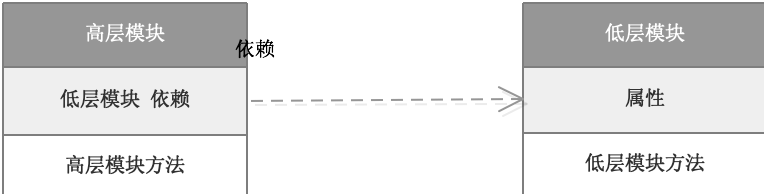
\includegraphics[width=0.5\textwidth]{beIOC.png}}\quad
\subfloat[使用 IoC 后]{\centering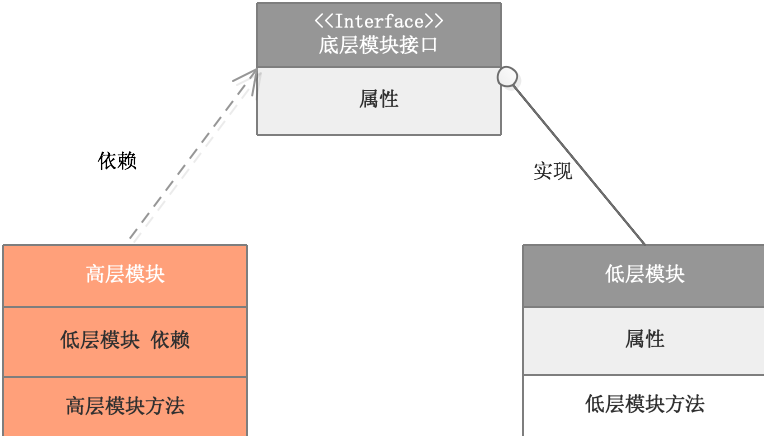
\includegraphics[width=0.5\textwidth]{afIOC.png}}
\caption{使用 IoC 前后 UML 图}
\label{fig:beforeAndAfter}
\end{figure}

Spring 的控制反转容器是通过依赖注入 (Dependency Injection, DI) 实现的。如图 \ref{fig:DI} 所示,依赖注入即高层模块在使用低层依赖时,不是自己讲低层模块实例化而是向控制反转容器申请一个已创建好的依赖对象。这样高层模块与低层模块间的耦合被降低了,对于低层模块的改变对高层模块产生的影响也变小了。同时,由于低层模块由容器创建,我们就可以轻松地实现单例模式等设计模式,进一步简化了开发也提高了系统的性能。

\begin{figure}[!ht]
    \centering
    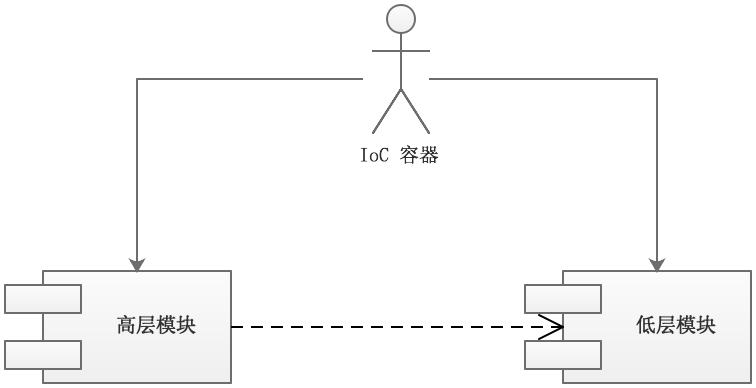
\includegraphics[width=0.6\textwidth]{IoC.png}
    \caption{Spring 依赖注入作用}
    \label{fig:DI}
\end{figure}

Spring 框架通过 BeanFactory 实现了最基本的控制反转功能,并且在 BeanFactory 之上提供了更先进的控制反转容器实现,即 ApplicationContext。BeanFactory 是基础类型的 IoC 容器,提供完整的 IoC 服务支持。 ApplicationContext 是高级的 IoC 容器,提供了诸如 Bean 生命周期管理、统一资源处理以及 AOP 支持等功能。通过使用 Spring 框架提供的 IoC 容器,我们可以轻松地使用控制反转构建应用系统。

\subsection{Spring AOP 框架}

在一个应用系统中存在着一些许多模块公用的功能,如:日志记录、安全检查以及事务功能等。这些公用功能如果处置不当就会造成系统的代码冗余度增加和耦合性上升,例如:要在系统中增加一次日志记录,我们就必须在所有的模块中加入相同的代码,着无疑是非常低效的。对此,我们可以使用面向切面编程 (Aspect Oriented Programming) 来解决这一问题。

\begin{figure}[!ht]
    \centering
    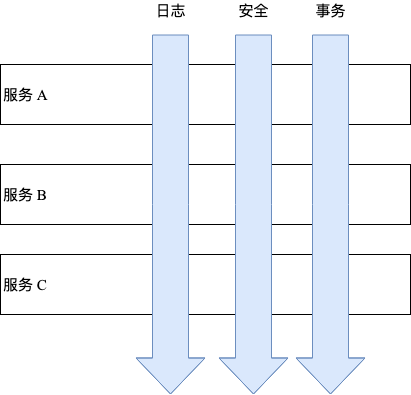
\includegraphics[width=0.6\textwidth]{AOP.png}
    \caption{面向切面编程中的横切关注点}
    \label{fig:AOP}
\end{figure}

如图 \ref{fig:AOP} 所示,面向切面编程可以将系统中的公共功能抽象成为许多称之为横切关注点的功能模块,例如:日志记录功能就是一个横切关注点。系统中需要使用这些公共功能的地方称之为连接点 (Joinpoint) 。在系统运行时面向切面编程框架会将横切关注点织入连接点中,这样系统就可以使用所有的公共功能,减少了系统的冗余代码与耦合性。

Spring 框架中的面向切面编程功能由动态代理实现,源于设计模式中的代理模式。如图 \ref{fig:Proxy} 所示,代理模式的作用是为其他对象提供一种代理以控制对这个对象的访问。代理处于访问者与被访问者之间,隔离两者的直接交互。在代理将访问者的访问请求传递给被访问者时,代理可以添加一部分额外的功能,如安全检测。因此,代理模式可以有效地增强系统的灵活性与安全性。动态代理的实现还要依靠 Java 提供的反射功能。反射功能雨荨我们在 Java 程序的运行期间动态载入类、创建对象以及生成代理。通过实现代理模式、使用反射机制,我们就可以创建出动态代理系统,实现面向接口编程。

\begin{figure}[!ht]
    \centering
    \includegraphics[width=0.6\textwidth]{Proxy.png}
    \caption{代理模式 UML 图}
    \label{fig:Proxy}
\end{figure}

Spring AOP 的设计遵循了 8/2 原则,即通过 20\% 的代码实现 AOP
 框架 80\% 的功能。因此Spring AOP 支持的 AOP 功能是不完全的,例如 Spring AOP 不支持属性级别的拦截等。系统运行时,我们在系统中定义所有的切面、连接点都会被 Spring AOP 拼装起来,这个操作被称为织入。织入时,Spring 会自动生成切面的代理包装类,通过代理包装类将切面织入代码中。Spring AOP 框架为我们提供了 AOP 的大部分功能,同时我们也可以整合使用 AspectJ 等框架来获取 Spring AOP 不支持的功能。
 
 \subsection{Spring 事务管理功能}
 
 事务管理的作用是保证应用系统在操作数据库时不会对数据的正确性产生破坏,具体的事务定义将在下文介绍。在 Spring 框架中,我们通常使用声明式的方式使用事务,事务也是一个常用的 AOP 中的横切关注点。通常情况下使用事务,我们需在每次访问数据库前声明事务开始,在事务正常结束后进行结束事务操作,在事务异常结束后进行事务的回滚。Spring 框架使用 AOP 来处理事务,通过在运行时将事务代码织入应用中来简化开发。
 
 我们在需要使用事务的地方使用 @Transactional 注解即可开启声明式事务功能,开启声明式事务功能后 Spring 并不直接管理事务,而是提供多种事务管理器,由它们将事务的具体管理委派给具体使用的各种持久化框架。我们也可以通过这些事务管理器进行事务属性的配置。事务属性主要包括:隔离级别、传播行为、回滚规则、是否只读以及超时时间等。通过注解使用声明式事务对于简化数据访问层的开发具有较大的意义。


\section{数据库的原理与设计}

本次设计采用 MySQL 作为系统主数据库、Redis 作为缓存数据库。

\subsection{MySQL 原理}
MySQL 是一个开源的关系型数据库管理系统。MySQL 非常的灵活,可以适应多种运行场景,例如:MySQL 既可以嵌入在程序中运行也可以支持数据仓库、在线处理系统等应用。

\subsubsection{关系型数据库}
关系型数据库是支持关系模型的数据库系统。关系模型非常的简单,只包含单一的数据结构 --- 关系。一个关系是一张二维表,可以由多个域的笛卡尔积表示。域是一组具有相同数据类型的值得集合。如一个班中所有学生的年龄的集合就是一个域。

笛卡尔积是一种域上的集合运算,其定义为:

\begin{equation}
\label{eq:Descartes}
D_1 \times D_2 \times \cdots \times D_n = {(d_1, d_2, \cdots, d_n) | d_i \in D_i, i=1, 2, \cdots, n}
\end{equation}

其中,每一个元素 $(d_1, d_2, \cdots, d_n)$ 为一个元组。笛卡尔积可以表示一个二维表,表中的一行对应笛卡尔积中的一个元组。$D_1 \times D_2 \times \cdots \times D_n$ 的子集为在域 $D_1, D_2, \cdots, D_n$ 上的关系。

每一个关系中都存在一些特殊的属性。若关系中某一属性组可以唯一标志该元组,而其任意子集均无此性质,则该属性组为这个关系的候选码。任意包含在至少一个候选码中的属性为主属性,不包含在所有候选码中的属性为非主属性。在任意关系表中不可能存在具有相同候选码的两个或多个元组。

关系数据库中,关系模式是关系的类型,关系是关系模式的实例。关系模式中主要包含关系中有哪些属性、关系中有哪些域以及域与属性的映射关系。关系模式可以表示为 $R(U, D, DOM, F)$,其中 $R$ 为关系名,$U$ 为属性名的集合,$D$ 为域的集合,$DOM$ 为属性与域的映射,$F$ 为属性间的依赖关系。

关系数据模型中也具有许多对于关系的操作,这些操作可以分为两类:集合操作和关系专用的操作。集合操作包括:并 (union, $\cup$ ) 、差 (except, $-$ ) 、交 (intersection, $\cap$ ) 、除 (divide, $\divide$ ) 和笛卡尔积 (Descartes Product, $\times$ )。关系专用操作包括:选择 (select, $\sigma$) 、投影 (project, $\Pi$) 以及连接 (join, $\join$)。其中,选择、投影、并、差、笛卡尔积是基本操作。其他的操作与基本操作关系如下:


\section{监控摄像头部署方案的评价指标}

监控摄像头的部署方案包括摄像头的数量以及部署位置。摄像头的部署位置会影响监控场景的完整性、监控画面的光线质量以及监控目标的呈现角度。而监控摄像头数量受成本预算的限制,不可能无限增加,因此在预算有限的约束下,如何设计监控摄像头的部署位置,使得监控效果最优,便成为一个值得研究的问题。在研究优化问题之前,需要定义监控摄像头部署方案的评价指标$\mathcal{E}$。

监控效果的优劣可以定义为在当前的监控方案下,跨摄像头追踪特定行人的能力。当前在多摄像头多行人追踪(Multi-Target Multi-Camera Tracking,MTMC Tracking)领域主流的评价指标有多目标跟踪准确度($\mathit{MOTA}$)~\cite{ristani2016MTMC}和识别F~值($\mathit{IDF_1}$)~\cite{ristani2016MTMC}。

\subsection{多目标跟踪准确度($\mathit{MOTA}$)}

多目标跟踪准确度(Multiple Object Tracking Accuracy,$\mathit{MOTA}$)是衡量多目标追踪效果的常见指标。对于一段视频,其画面帧的总数为$T$,那么该段视频的多目标追踪准确度($\mathit{MOTA}$)的定义为:
\begin{equation}
\label{eq:mota}
\mathit{MOTA}=1-\frac{\mathit{FP}+\mathit{FN}+\Phi}{T}
\end{equation}
其中$\mathit{FN}$是视频所有帧中将负样本预测为正的总数,$\mathit{FP}$是视频所有帧中将正样本预测为负的总数,$\Phi$是预测序列中标签跳变的次数。$\mathit{MOTA}$指标的值域为$(-\infty,1]$,越接近1代表跟踪的效果越好。

\subsection{识别F值($\mathit{IDF_1}$)}

相比与$\mathit{MOTA}$中更多地关注目标人群的召回率以及目标追踪的稳定性,识别F值(Identification F-Score,$\mathit{IDF_1}$)更关注多摄像头多行人追踪过程中,行人标签的准确率。对于一段总帧数为$T$的视频,其识别F值($\mathit{IDF_1}$)定义为:
\begin{equation}
\mathit{IDF_1}=\frac{2\times\mathit{IDTP}}{2\times\mathit{IDTP}+\mathit{IDFP}+\mathit{IDFN}}
\end{equation}
其中$\mathit{IDTP}$是视频所有帧中将人物标签预测准确的总和,$\mathit{IDFP}$是视频所有帧中将正样本的人物标签预测错误的总和,$\mathit{IDFN}$是视频所有帧中将负样本的人物标签预测错误的总和。

\subsection{评价指标与当前的数据库结合}

结合本项目的实际情况,以及第一次预拍摄收集到的数据集的特点,将原始的17个摄像头中的第1个作为行人重识别算法的图库图片来源,其余16个摄像头按照物理位置和拍摄画面分为$G=5$组,每组摄像头个数为2至4个不等,定义$N=16$为待分配的摄像头总数,第$i$组的摄像头个数为$C_i$,同一组内摄像头大致拍摄到同一个物理位置,代表人物监控追踪场景中重点关注的位置。第$i$组的第$j$个摄像头定义为$c_{i,j}$,摄像头$c_{i,j}$的画面帧集合为$\mathcal{I}_{c_{i,j}}$。假设在预算有限的前提下,每个位置(每个分组)只能选择1个摄像头,如何从组内选择合适的摄像头,使得监控效果最佳,便是需要解决的问题。该优化问题可以用数学语言形式化表示为:
\begin{equation}
\max \left\{\mathcal{E}\left[\mathcal{F}\left(\sum_{i=1}^G \mathcal{I}_{c_{i,j}}\right)\right]\,\middle\vert\, 1\leq i \leq G, 1\leq j \leq C_i\right\}
\end{equation}
其中$\mathcal{I}_{c_x}+\mathcal{I}_{c_y}$表示摄像头$c_x$的视频数据与摄像头$c_y$的视频数据在时序上依次拼接。$\mathcal{E}[\mathcal{F}(\mathcal{I})]$表示对视频数据$\mathcal{I}$做多目标跟踪准确度($\mathit{MOTA}$)或识别F值($\mathit{IDF_1}$)评估。

\section{强化学习模型}

强化学习(Reinforcement Learning)是近年来十分流行的人工智能算法,相比于监督学习(Supervised Learning),强化学习不需要整个环境(Environment)所有情况的监督信息,只需要环境在某种特定的情况下给出相应的反馈(Reward)。在很多现实问题当中,优化空间的状态个数可能是个非常大的数字,且很证明是否收集到足够多样本,可以用来近似代表位置环境状态的分布。同时,在围棋问题~\cite{silver2016mastering}中,各状态空间很难用监督的方法给每个状态评估价值,而强化学习只需要环境在每次动作(Action)之后给出相应的反馈,即可逐渐向更优的方向前进。强化学习也不属于无监督学习(Unsupervised Learning),无监督学习对于出现在测试集却不在训练集的样本没有处理能力,只能错误地分到已有的类中,而强化学习可以应对没有遇到的情况。

强化学习模型中的一般形式是一个智能体(Agent)在一个客观的环境(Environment)中,每一个时刻处于一个状态(State),当前状态存在一个短期价值和长期价值,短期价值可以是采取某种动作(Action)之后得到的反馈(Reward),长期价值(Value)则表示当前状态到最终状态能够得到的所有反馈总和的最大值。智能体根据当前状态的短期或长期价值和某种策略(Policy)采取某种动作,可立刻得到得到环境的反馈(Reward),并据此按照状态转移规则转移到下一个状态。在本项目中,根据要解决的具体问题,将上述概念相应定义如下:

当前的状态的集合$S=\left\{\boldsymbol{s}\,\middle\vert\,\boldsymbol{s}\in\mathbb{R}^{N}, s_i\in\{0, 1\}\right\}$,其中$s_i=1$表示选择了第$i$个摄像头。智能体可以采取的动作集合为$A=\left\{\boldsymbol{a}\,\middle\vert\,\boldsymbol{a}\in\mathbb{R}^N,a_i \in \{0,1\}\right\}$,按照策略 $P$ 来选择动作, 1 表示选择该摄像头,0表示不选该摄像头。在本项目中,进行了动作之后, 状态是确定的,不存在一个动作可能导致几个不同的后续状态的情况,即状态转移概率 $\pi\left(\boldsymbol{s}^t\,\middle\vert\,\boldsymbol{s}^{t-1}, \boldsymbol{a}\right)\equiv1$。执行动作之后得到的反馈$r=\mathcal{E}\left[\mathcal{F}\left(\mathcal{I}^{(t+1)}\right)\right]-\mathcal{E}\left[\mathcal{F}\left(\mathcal{I}^{(t)}\right)\right]$,其中$\mathcal{I}^{(t)}$表示$t$时刻的视频数据,由$t$时刻的状态$\boldsymbol{s}^{(t)}$决定。当前状态 $S$ 的长期价值$V:\,S\mapsto\mathbb{R}^N$,是一个可学习的变量,代表智能体对于当前环境的认识程度。智能体应对当前状态的策略$P:\,V\mapsto A$,是长期价值 $V$ 到动作 $A$ 的映射,可以简单地用贪心的策略,即选择概率最高的 5 个摄像头。也可以用 Policy Network ,即深度神经网络来实现。在本项目中采用简单的贪心策略实现,如算法~\ref{alg:qlearning}~所示。

\begin{algorithm}[!htb]
    \caption{Q-Learning 算法求当前状态的长期价值}
    \label{alg:qlearning}
    \begin{algorithmic}[1]
        \Require 状态集合$S$、动作集合$A$、生命周期数$N$、学习率$\alpha$、远见性$\gamma$
        \Ensure 长期价值矩阵$Q$
        \Function {QLearning}{$S, A, N, \alpha, \gamma$}
            \State 随机初始化长期价值矩阵$Q$
            \For{$i=0\to N$}
                \State $\boldsymbol{s}^{(0)}\gets\boldsymbol{s}^\star$,$\boldsymbol{s}^\star$为从状态集合$S$中随机初始化的智能体的状态
                \State $t\gets1$
                \Repeat
                    \State $\boldsymbol{a}^{(t)}\gets \boldsymbol{a}^\star$,$\boldsymbol{a}^\star$为从动作集合$A$中随机选取的动作
                    \State $\boldsymbol{s}^{(t+1)}\gets \pi\left(\boldsymbol{s}^{(t)}, \boldsymbol{a}^{(t)}\right)$
                    \State $r^{(t)}\gets R\left(\boldsymbol{s}^{(t+1)},\boldsymbol{s}^{(t)}\right)$
                    \State $Q\left(\boldsymbol{s}^{(t)},\boldsymbol{a}^{(t)}\right)\gets(1-\alpha)\times Q\left(\boldsymbol{s}^{(t)},\boldsymbol{a}^{(t)}\right)+\alpha\times\left[r^{(t)}+\gamma\times\max_{\boldsymbol{a}'}Q\left(\boldsymbol{s}^{(t+1)}, \boldsymbol{a}'\right)\right]$
                    \State $\boldsymbol{s}^{(t)}\gets\boldsymbol{s}^{(t+1)}$
                    \State $t\gets  t+1$
                \Until{$\boldsymbol{s}^{(t)}=\boldsymbol{s}^{(0)}$}
            \EndFor
            \State\Return $Q$
        \EndFunction
    \end{algorithmic}
\end{algorithm}

按照以上定义,智能体的一个动作就是选择一个合法的摄像头部署方案。对于一个动作,它的反馈就是下一个状态的性能指标$\mathcal{E}$($\mathit{MOTA}$ 或 $\mathit{IDF_1}$)减去当前状态的性能指标。在反馈已知的前提下,适合用 Q-Learning~\cite{watkins1989learning} 算法。在Q-Learning算法中,智能体关于当前状态的长期价值表示为一个价值矩阵$Q$。Q-Learning算法首先随机初始化各个状态的长期价值,让智能体在环境中随机游走,每走一步会得到一个反馈,根据反馈更新当前状态的长期价值,直到收敛。智能体从而可学习出一个对于该环境的认知。在算法~\ref{alg:qlearning}~中最关键的算法在于如何更新长期价值$Q$,更新的公式中包含两个参数学习率$\alpha$和远见性$\gamma$,学习率$\alpha$表示$Q$的更新速度,远见性$\gamma$的取值范围为$(0, 1)$,表示智能体对于当前反馈与长远价值的重视程度,$\gamma$越大,代表越重视长远价值。

\section{面向CPU集群的分布式深度学习训练框架}

计算机集群是一种计算机组织的物理形态,它是由一组彼此连接的计算机组成的,这些计算机一般协同完成同一项计算任务。在同一集群中每台计算机的内部结构可以不同,特别地,若集群中每台计算机主要的算力提供者是CPU,那么称该集群为CPU集群。分布式计算是计算的一种工作方式,它将一个计算任务划分成多个子任务,每一个子任务与其它子任务相对独立,可以在时间上并行计算,以缩短计算时间。CPU集群提供了一组在物理上相对独立的计算机,所以可以很自然地考虑将分布式计算中的各个子任务部署到CPU集群中,充分利用CPU集群的计算资源。

深度神经网络模型的训练过程一般可分为前馈计算(Forward)、误差反向传播(Loss Backpropagation)和参数更新。其中前向计算和反向传播的计算量很大,而且可以针对不同的训练集进行同步计算,因此深度神经网络模型的训练过程在结构上很适合进行分布式训练。在本项目中,集群的数量$n=5$,每个节点属于天河二号的GPU分区,具备高性能的CPU和GPU计算资源,节点之间通过千兆网络连接,避免各节点的通信速度成为分布式计算的性能瓶颈。本项目中分布式训练架构如图~\ref{fig:dist}~所示。

\begin{figure}[!ht]
\centering
\includegraphics[width=0.7\textwidth]{dist}
\caption{分布式神经网络训练架构图}
\label{fig:dist}
\end{figure}

如图~\ref{fig:dist}~所示,在训练过程中将训练数据通过随机采样的方式平均分成$n$份,分别输入集群中的各计算机。每一台计算机内存中包含一个独立的深度神经网络模型,进行该份训练数据的前馈计算和反向传播计算,得到该批次训练数据在当前模型下的各参数梯度。参数服务器的计算任务是收集集群中各计算机回传的梯度,更新模型参数,并将新参数分发给各计算机,各计算机得到新参数后进行下一批次训练数据的计算。更新模型参数的方法为:
\begin{eqnarray}
\Delta W=\frac{1}{n}\sum_{i = 1}^{n}\Delta W_i \\
W=W-\eta\Delta W
\end{eqnarray}
其中$\eta$是参数的学习率。